\documentclass{report}
\usepackage[utf8]{inputenc}
\usepackage[a4paper, total={7in, 10in}]{geometry}
\usepackage{graphicx}
\usepackage[parfill]{parskip}
\usepackage{amsmath}
\usepackage{wrapfig}
\usepackage{subfig}
\usepackage{titlesec}

\titleformat{\chapter}[display]
{\normalfont\huge\bfseries}{\chaptertitlename\ \thechapter}{20pt}{\Huge}
\titlespacing*{\chapter}{0pt}{0pt}{40pt}


\graphicspath{ {./Images/} }
\setlength{\parindent}{0em}

\title{Computer Vision} 
\author{Xin Wang}

\begin{document}
\par
\maketitle
\medskip

\tableofcontents

%%%%%%%%%%%%%%%%%%%%%%%%%%%%%%%%%%%%%%%%%%%%%%%%%%%%%%%%%%%%%%%%%%%%%%%%%%%%%%%%%%%%%%%%%%%%
\chapter{Image Formation}

A digital image is formed from three components:
\begin{enumerate}
    \item Lighting 
    \item Reflectance 
    \item Optics and Sensors
\end{enumerate} 

\section{Lighting}

Lighting has several properties of concern:
\begin{itemize}
    \item Location 
    \item Intensity of light 
    \item Spectrum of light
\end{itemize} 

There are many different sources of light. Four commonly used models to describe
light sources are:
\begin{itemize}
    \item \textbf{Point Light Source}: The light is inside the scene at a
    specific location only and it shines light equally in all directions. An example
    is be a table lamp.
    \item \textbf{Area Light Source}: The light source comes from a rectangular
    area and projects light from one side of the rectangle. An example is a
    florescent light fixture in a ceiling panel. 
    \item \textbf{Sun Light Source}: The light is outside the scene and far
    enough away that all rays of light are basically from the same direction. 
    An example is the sun in an outdoor scene.
    \item \textbf{Spotlight Light Source}: The light is focused and forms a
    cone-shaped envelop as it projects out from the light source. An example is
    a spotlight in a theatre. 
\end{itemize}

\section{Reflectance}

\begin{wrapfigure}[10]{r}{0.45\linewidth}
\centering
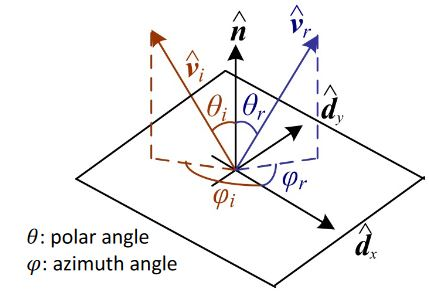
\includegraphics[width=6cm]{BRDF.JPG}
\caption{BRDF model}
\label{fig:myfig}
\end{wrapfigure}

A general model for modelling reflectance is the
\textbf{Bidirectional Reflectance Distribution Function (BRDF)}. The model
describes how much light arriving at incident direction is emitted in
reflected direction. 
$$
f_r\left(\theta_i, \sigma_i, \theta_r, \sigma_r, \lambda\right) = \frac{dL_r}{dE_i}
$$
where:
\begin{itemize}
    \item $\theta_i$ and $\sigma_i$: Incident direction
    \item $\theta_r$ and $\sigma_r$: Reflected direction
    \item $\lambda$: Wavelength
    \item $dL_r$: Output power 
    \item $dE_i$: Input power 
\end{itemize}

\pagebreak

Considering the two ideal cases of reflection: \textbf{Diffuse reflection} and
\textbf{Specular reflection}
\begin{itemize}
    \item \textbf{Diffuse reflection}: 
    \begin{figure}[h!]
        \centering
        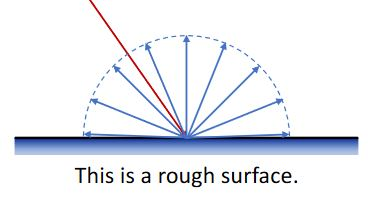
\includegraphics[width=.2\linewidth]{Diffuse reflection angle.JPG}
        \qquad
        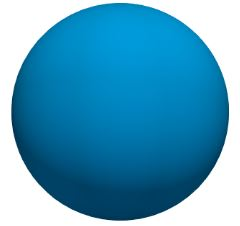
\includegraphics[width=.1\linewidth]{Diffuse reflection view.JPG}
    \end{figure}

    The light is scattered uniformly in all directions so the BRDF is constant:
    $$
        f_r\left(\theta_i, \sigma_i, \theta_r, \sigma_r, \lambda\right) = f_r(\lambda)
    $$

    This effect on the viewed image is similar to the appearance of a rough
    surface.
    
    \item \textbf{Specular reflection}: 
    \begin{figure}[h!]
        \centering
        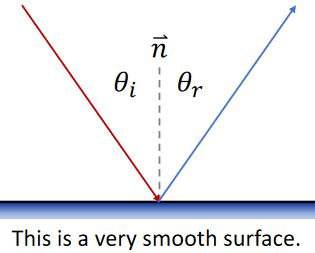
\includegraphics[width=.15\linewidth]{Specular reflection angle.JPG}
        \qquad
        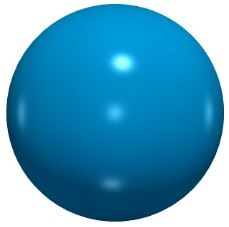
\includegraphics[width=.1\linewidth]{Specular reflection view.JPG}
    \end{figure}

    The light is reflected in a mirror-like fashion. The reflection and incident directions are symmetric with respect to the
    surface normal $\vec{n}$: $\theta_r = \theta_i$
\end{itemize}

For the majority of cases in the real world, there is a combination of
\textbf{diffuse reflection}, \textbf{specular reflection} and \textbf{ambient
illumination}. Ambient illumination accounts for general illumination which may be
complicated to model such as the inter-reflection between walls in a room and
distant light sources as seen in sunny outdoor environments.

This observation is formally state in the \textbf{Phong Reflection Model} which
is an empirical model in computer graphics that describes how a surface reflects
light as a combination of ambient, diffuse and specular components. 
\begin{figure}[h]
    \centering
    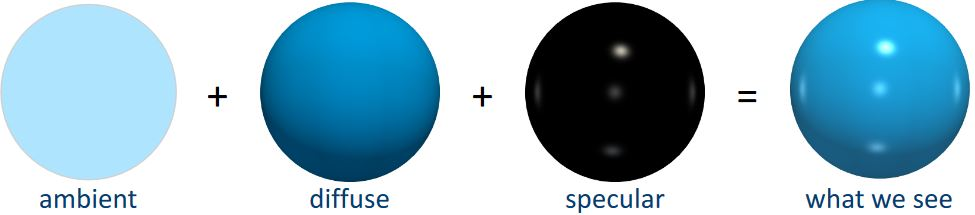
\includegraphics[width=10cm]{Phong reflection model.JPG}
\end{figure}

\subsection{Computer graphics}

There is an unique relationship between computer graphics and computer vision
similar to the relationship of writing and reading. Computer graphics is
concerned with generating images while computer vision is concerned with
intepreting images. 

This relationship is particularly valuable as computer graphics in
photorealistic games can be used to generate data i.e. images + labels for
training computer vision algorithms. 

\section{Optics}

Camera sensors imitates the human eye which are human sensors. In the human eye,
there are two types of neural cells in the retina: 
\begin{itemize}
    \item \textbf{Cone cells}: Colour vision and functions in the bright light. 
    \item \textbf{Rod cells}: More sensitive to the light but monochromatic and
    functions in the dim light like night time. 
\end{itemize}

Camera sensors are very much the same: \textbf{Charge-coupled Device (CCD)} and
\textbf{Complementary Metal-oxide Semiconductor (CMOS)}.

\subsection{Colour Filter Arrays (CFA)}

A color filter array (CFA) or color filter mosaic (CFM) is a mosaic of tiny
color filters placed over the pixel sensors of an image sensor to capture color
information.  

The most common CFA is the most single-chip digital image sensors used in
digital cameras to create a colour image is the \textit{Bayer Filter Mosaic}.
The Bayer Filter Mosaic is arraged to mimic the human eyes i.e. most sensitive
to green light with $50\%$ green, $25\%$ red and $25\%$ blue.

The RGB of different cameras may be different, i.e. with different sensitivities
to wavelengths. This different colour sensitivity is why the same picture with
different cameras would look different.

\subsection{Bayer Colour Filter}

With its arrangement, only one colour is available at each pixel. The other two
colours can be interpolated from neighbouring pixels. Through this
interpolation at each pixel, the RGB values can be obtained. 
\begin{figure}[h]
    \centering
    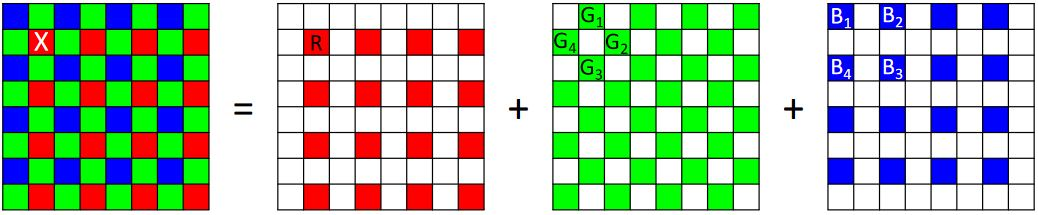
\includegraphics[width=10cm]{Bayer colour filter.JPG}
    \caption{Bayer colour filter and interpolation}
\end{figure}

\subsection{Demosaicing}

A demosaicing algorithm is a digital image process used to reconstruct a full
colour image from incomplete colour samples output from an image sensor overlaid
with a CFA.

A simple method is bilinear interpolation where the red value of a non-red pixel
is computed as the average of the two or four adjacent red pixels, and similarly
for blue and green.  
\begin{figure}[h]
    \centering
    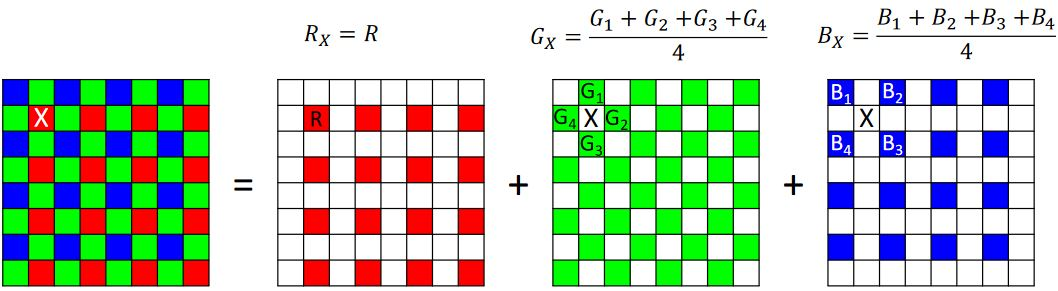
\includegraphics[width=10cm]{Demosaicing algorithm.JPG}
\end{figure}

\subsection{Colour spaces}

\begin{wrapfigure}[10]{r}{0.35\linewidth}
    \centering
    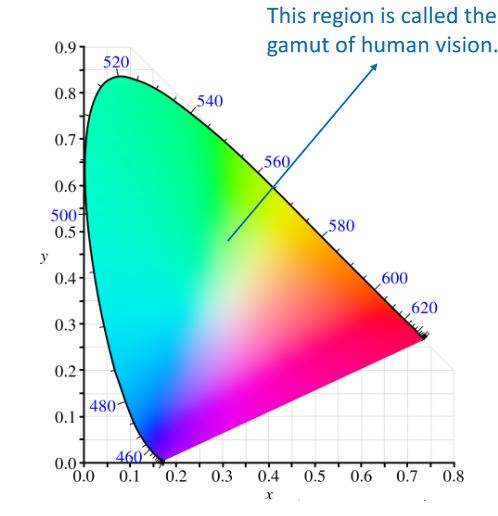
\includegraphics[width=5cm]{Colour space repre.JPG}
    \caption{CIE 1931}
\end{wrapfigure}

Colour spaces are mathematical models describing the way colours can be
represented. Colour spaces can be seen as a box containing all possible colours that can be
produced by mixing primary colours of RGB. 

The CIE 1931 XYZ was created by the International Commission on Illumination and
represents the colour space using the primary colours X, Y and Z. 
\begin{align*}
    x &= \frac{X}{X+Y+Z} \\
    y &= \frac{Y}{X+Y+Z} \\
    z &= \frac{Z}{X+Y+Z}
\end{align*}

There are various different forms colour spaces such as sRGB, HSV and CMYK.  All
these colour spaces can represent the same colour, but using different
primary colours or coordinate systems.

\subsection{Quantisation}

Quantisation is the process that maps continuous signal to discrete signal. For
colours, color quantization reduces the number of colors used in an image. This
is important for displaying images on devices that support a limited number of
colors and for efficiently compressing certain kinds of images.

It is important to note that numerical errors occur during quantisation,
which depends on the number of bits used. The more bits, the less quantisation
error.

%%%%%%%%%%%%%%%%%%%%%%%%%%%%%%%%%%%%%%%%%%%%%%%%%%%%%%%%%%%%%%%%%%%%%%%%%%%%%%%%%%%%%%%%%%%%
\chapter{Image Filtering}

The goal of using filters is to modify or enhance image properties and/or to
extract valuable information from the pictures such as edges, corners, and
blobs.

There are various types of image filters such as:
\begin{itemize}
    \item Identity filter
    \item Low-pass/Smoothing filters: Moving average filter or Gaussian filter 
    \item High-pass/Sharpening filters 
    \item Denoising filter: Median filter
\end{itemize}

\section{Smoothing Filters: Moving Average Filter}

A moving average filter moves a window across the signal and calculates the
average value within the window. A \textbf{filter kernal} is specified to
indicate what values are averaged in the moving average filter. A filter
kernal \footnote{https://en.wikipedia.org/wiki/Kernel\_(image\_processing)}
is a small matrix used for blurring, sharpening, edge detection etc. 

In images, the moving average filter removes high frequency signal e.g. noise or
sharpness. This operation results in a smooth but blurry image. For example,
consider a \textbf{box blur} kernal and its effect:

\begin{minipage}{7in}
    \centering
    \raisebox{-0.5\height}{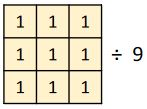
\includegraphics[height=0.5in]{Box blur.JPG}}
    \hspace*{.2in}
    \raisebox{-0.5\height}{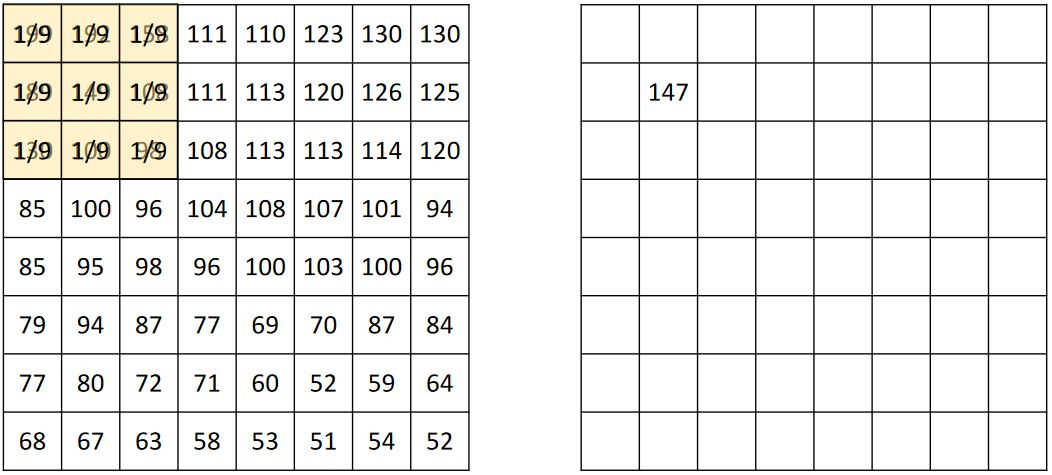
\includegraphics[height=1.5in]{Box blur calculation.JPG}}
\end{minipage}

Due to the nature of this method of calculations, the output image will be
smaller than the input image. The boundary pixels are generally dealt with using
padding of various methods such as constant value, mirroring values etc. The
following example uses 0 padding for its boundary pixels. 

\begin{minipage}{7in}
    \centering
    \raisebox{-0.5\height}{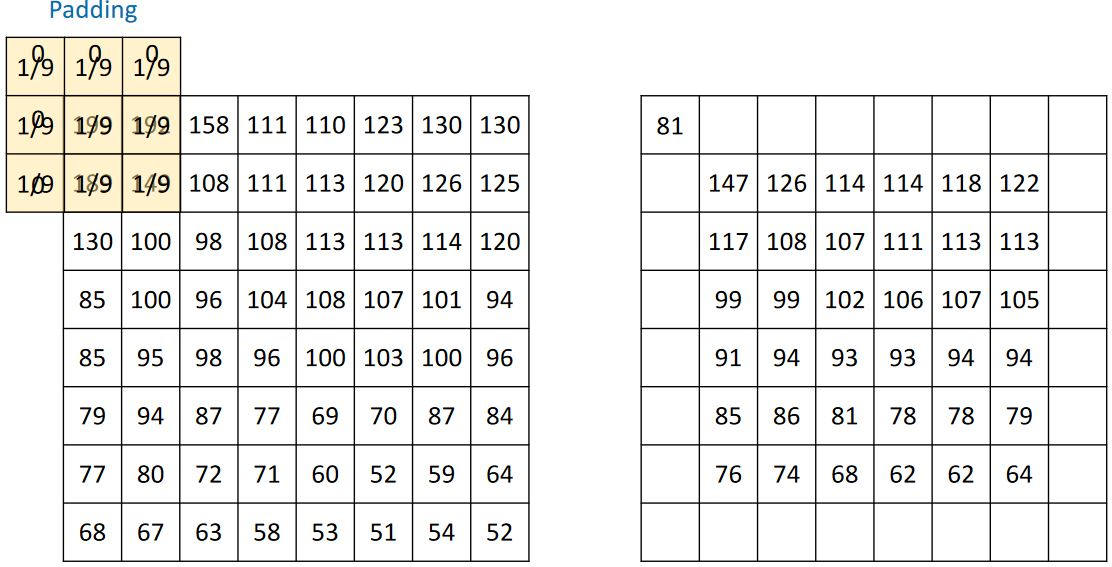
\includegraphics[height=1.5in]{Zero padding.JPG}}
    \hspace*{.2in}
    \raisebox{-0.5\height}{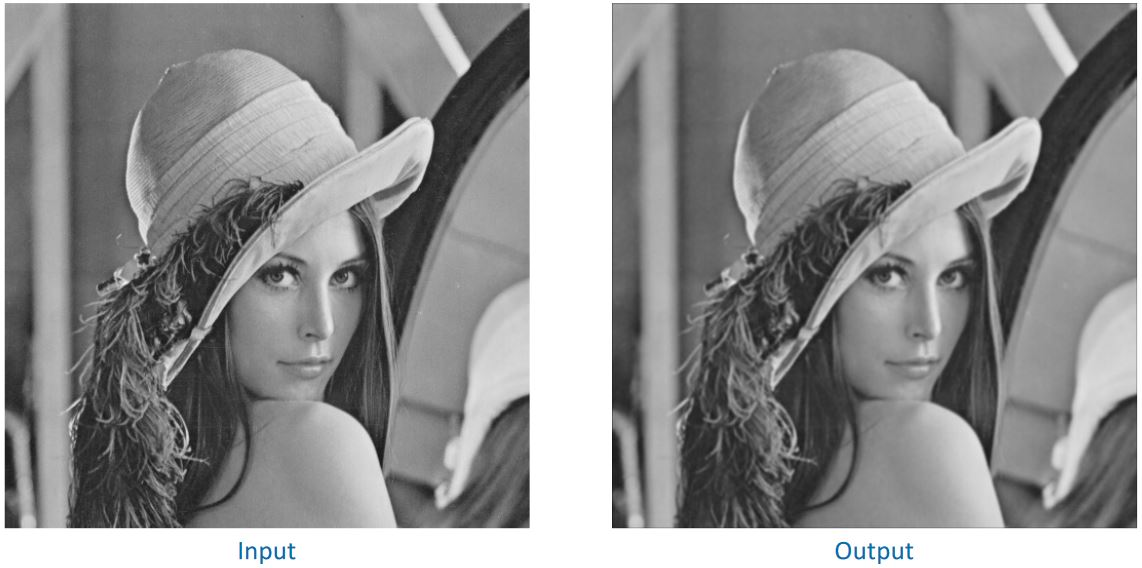
\includegraphics[height=1.5in]{Blur images.JPG}}
\end{minipage}

By increasing the size of the kernal e.g. into a $7 \times 7$ matrix, the image
will become blurrier. 

\vfill

\subsection{Brute Computational Complexity}

Note that: \textit{Image size}: $N \times N$ where $N$ is the number of pixels and
\textit{Kernal size}: $K \times K$ where $K$ is size of the filter kernal matrix 
\begin{itemize}
    \item There are $N^2$ pixels 
    \item At each pixel, there are $K^2$ multiplications and $K^2 - 1$ summations.
    \item In total, there are: $N^2 K^2$ multiplications and $N^2(K^2 - 1)$
    summations 
    \item Complexity is: $O(N^2 K^2)$
\end{itemize}

\subsection{Separable filter}

If a big filter can be separated as the consecutive operation of two small
filters, then the first filter can be applied to the the input image then the
second filter. For example, consider the previous blur filter kernal divided
into two smaller filters:
\begin{figure}[h]
    \centering
    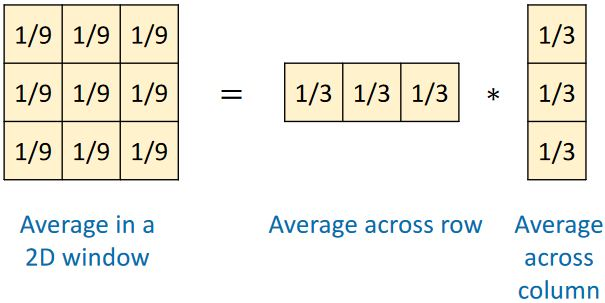
\includegraphics[width=6cm]{Blur separable filter.JPG}
\end{figure}

This calculation procedure results in the same result as the previous result:

\begin{minipage}{7in}
    \centering
    \raisebox{-0.5\height}{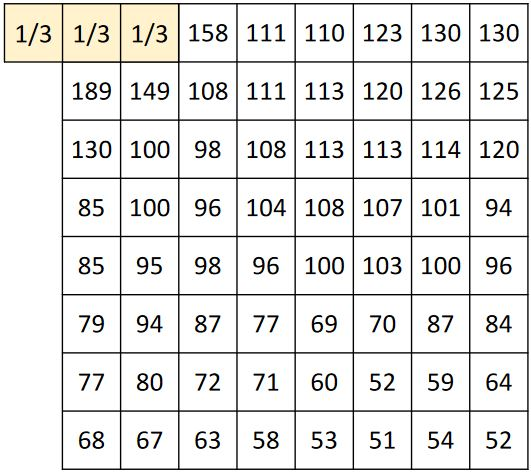
\includegraphics[height=1.5in]{X separable filter 1.JPG}}
    \hspace*{.2in}
    \raisebox{-0.5\height}{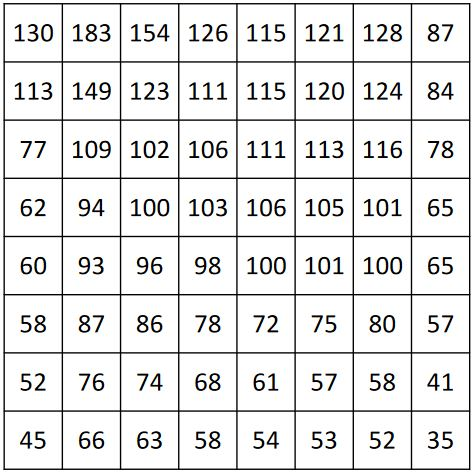
\includegraphics[height=1.5in]{X separable filter 2.JPG}}
\end{minipage}

\begin{minipage}{7in}
    \centering
    \raisebox{-0.5\height}{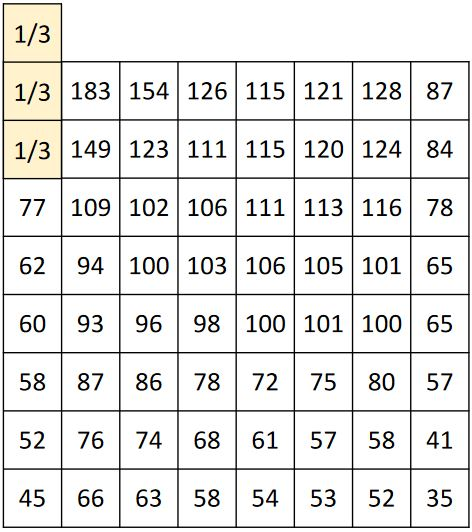
\includegraphics[height=1.5in]{Y separable filter 1.JPG}}
    \hspace*{.2in}
    \raisebox{-0.5\height}{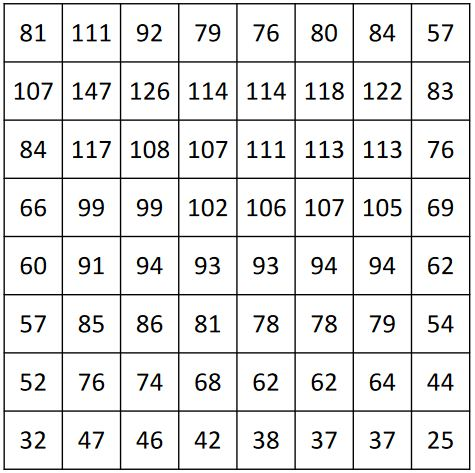
\includegraphics[height=1.5in]{Y separable filter 2.JPG}}
\end{minipage}

\subsection{Separable filter complexity}

Note that: \textit{Image size}: $N \times N$ where $N$ is the number of pixels
and there are two filter kernals: $1 \times K$ and $K \times 1$.
\begin{itemize}
    \item There are $N^2$ pixels 
    \item At each pixel, there are $K$ multiplications and $K - 1$ summations.
    \item In total, there are: $2N^2 K$ multiplications and $2N^2(K - 1)$
    summations 
    \item Complexity is: $O(N^2 K)$ which is faster than the previous $O(N^2 K^2)$
\end{itemize}

\section{Identity Filter}

The \textbf{Identity Filter Kernal} simply returns the same value of the image
i.e. the input and output image is the same.

\section{Smoothing Filters: Gaussian Filter}

The Gaussian Filter uses a 2D Gaussian Distribution as its filter kernal:
$$
    h(i,j) = \frac{1}{2\pi \sigma^2} e^{- \frac{i^2 + j^2}{2\sigma^2}}
$$

The 2D Gaussian filter is a separable filter, equivalent to two 1D Gaussian
filters with the same $\sigma$, one along x-axis and the other along y-axis:
\begin{align*}
    h(i,j) &= h_x(i) * h_y(j) \\
    h_x(i) &= \frac{1}{\sqrt{2\pi}\sigma}e^{-\frac{i^2}{2\sigma^2}}
\end{align*}

\section{High-pass Filters}

There are various methods of designing high-pass filters including using
low-pass filters as seen in Design 1.
\begin{figure}[h]
    \centering
    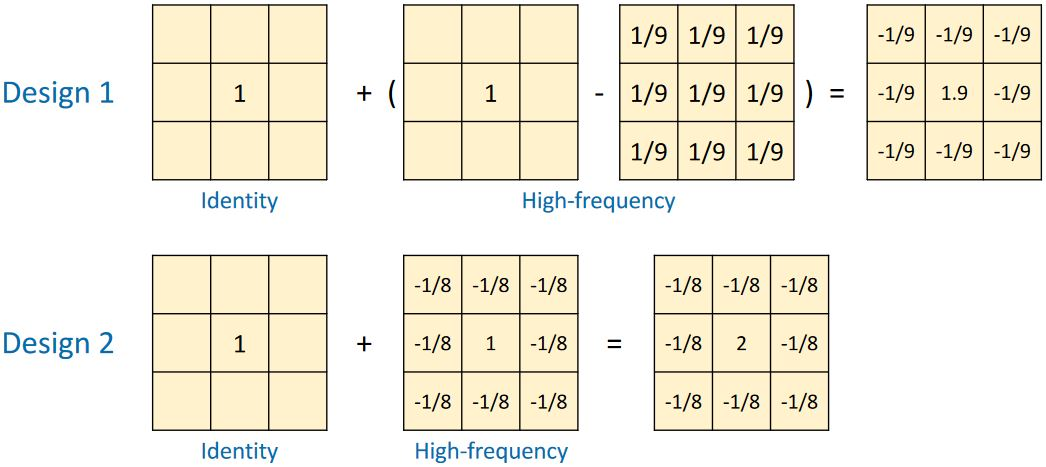
\includegraphics[width=10cm]{High pass.JPG}
\end{figure}

\section{Denoising Filters: Median Filter}

Median filters are non-linear filters that is often used for denoising an image.
A common method of performing median filter is to move the sliding window and
replacing the centre pixel using the \textit{median value} in the window.
\begin{figure}[h]
    \centering
    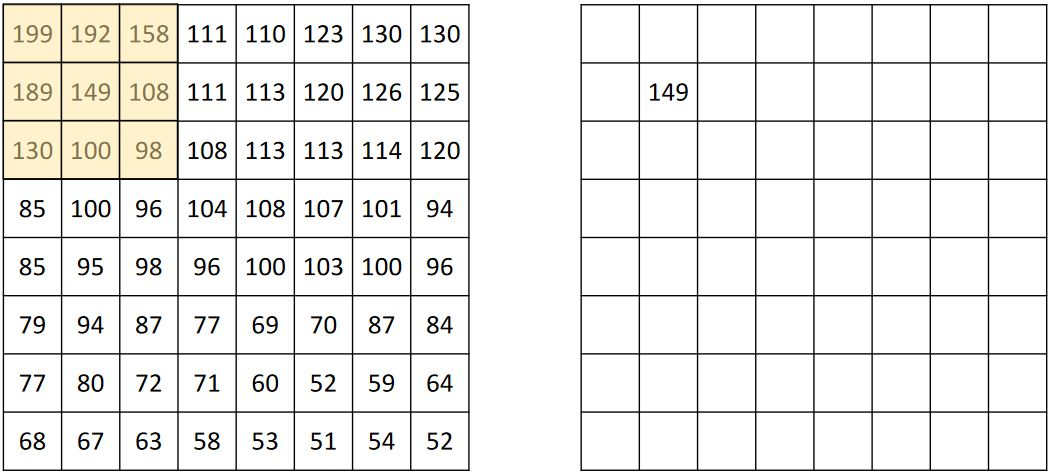
\includegraphics[width=10cm]{Median filter.JPG}
\end{figure}

%%%%%%%%%%%%%%%%%%%%%%%%%%%%%%%%%%%%%%%%%%%%%%%%%%%%%%%%%%%%%%%%%%%%%%%%%%%%%%%%%%%%%%%%%%%%
\chapter{Image Filtering II}

The concept of filtering can be described mathematically for example: 
\begin{figure}[h]
    \centering
    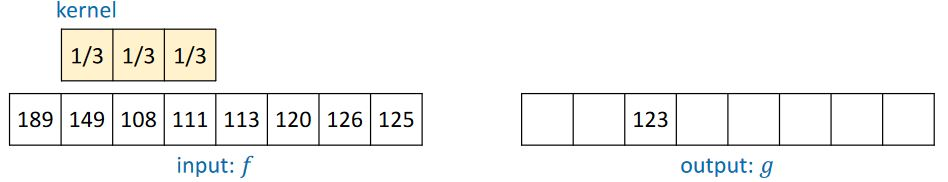
\includegraphics[width=8cm]{Filter_mathematical_example 1.JPG}
\end{figure}
where this operations can be described as:
$$
    g[n] = \frac{1}{3} . f[n-1] + \frac{1}{3} . f[n] + \frac{1}{3} . f[n+1]
$$

This concept of describing filters mathematically is extensively used in Signal
Processing where it describes filters as:
\begin{center}
    \textit{A device/process '$h$' that removes unwanted components/features from a input
    signal '$f$' and generates an output signal '$g$'}
\end{center}

\section*{Impulse Response}

Impulse responses are used to mathematically describe a filter. The impulse
response $h$ is the output of a filter when the input is an impulse signal $\delta$. 
\begin{figure}[h]
    \centering
    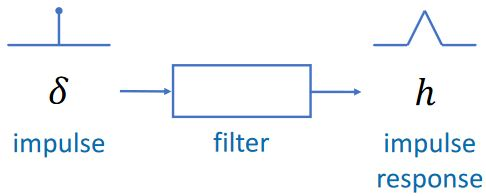
\includegraphics[width=5cm]{Impulse response.JPG}
\end{figure}

\begin{itemize}
    \item \textbf{Continuous signal}: An impulse signal is the \textit{Dirac
    Delta function} $\delta(x)$:
    \begin{gather*}
        \delta(x) = \begin{cases}
            +\infty & \text{if } x = 0 \\
            0 & \text{otherwise}
        \end{cases} \\
        \int^{\infty}\delta (x) dx = 1
    \end{gather*}

    \item \textbf{Discrete signal}: An impulse signal is the \textit{Kronecker
    function} $\delta[i]$: 
    \begin{gather*}
        \delta[i] = \begin{cases}
            1 & \text{if } i = 0 \\
            0 & \text{otherwise}
        \end{cases}
    \end{gather*}
\end{itemize}

The impulse response $h$ completely characterises a \textit{linear
time-invariant} filter. Because any input signal can be form using impulses, if
one knows how the system may response to one impulse then you know how the system
will response to many impulses. 

\pagebreak

\textbf{Time-invariant system}: If a filter is a \textit{time-invariant system},
when the input is shifted by time step $k$, the output will also shift by $k$.
In the following example, note how the impulse response for $f[n]$ and $f[n-2]$
are the same but only shifted by $2$ in a LTI system.
\begin{figure}[h]
    \centering
    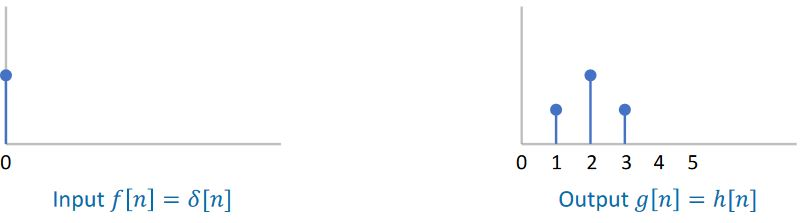
\includegraphics[width=8cm]{Impulse response shift 1.JPG} \\
    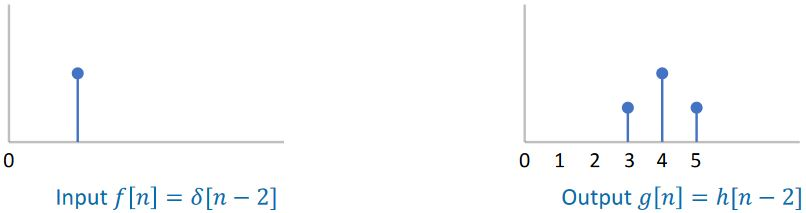
\includegraphics[width=8cm]{Impulse response shift 2.JPG}
\end{figure}

\textbf{Linear system}: If a filter is a \textit{linear system},
when the input is multiplied by $k$, the output will also by multiplied by $k$.
\begin{figure}[h]
    \centering
    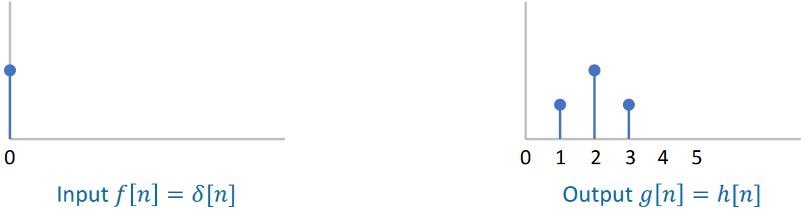
\includegraphics[width=8cm]{Linear response.JPG} \\ 
    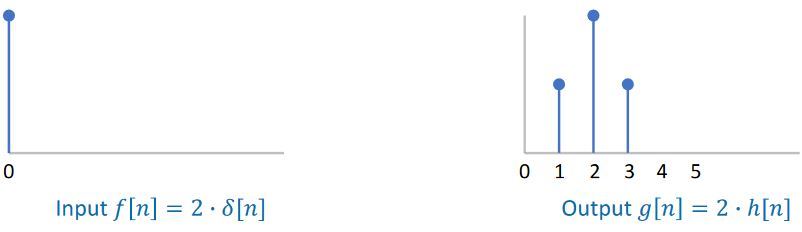
\includegraphics[width=8cm]{Linear response 2.JPG} 
\end{figure}

Similarly, if a filter is a linear system, when combining two input signals linearly,
their outputs will also be combined linearly.
\begin{figure}[h]
    \centering
    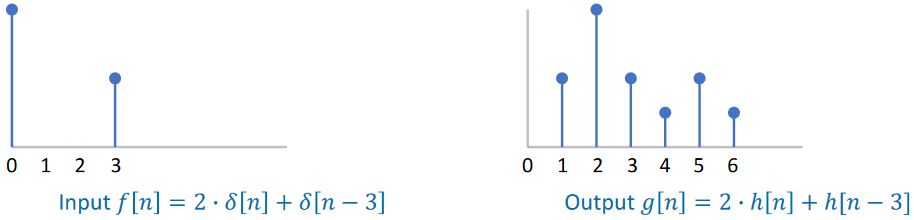
\includegraphics[width=8cm]{Linear combined.JPG}
\end{figure}

\section{Convolution and Linear Time-invariant System (LTI)}

For a linear time-invariant system, the impulse response $h$ completely
characterises how the LTI system works. The output $g$ can be described as the
\textit{convolution} between input $f$ and impulse response $h$:
$$
    g[n] = f[n] * h[n] = \sum_{m=-\infty}^\infty f[m]h[n-m]
$$

Convolutions are usually implemented by: 
\begin{enumerate}
    \item Flip the kernel 
    \item Multiply the signal with the flipped kernel 
    \item Sum over the support of the kernel 
\end{enumerate}
$$
    \sum_{m=-\infty}^\infty f[m]h[n-m] = \sum_{m=-\infty}^\infty f[n+m]h[-m]
$$

\subsection{Propoerties of convolution}
\begin{itemize}
    \item \textbf{Commutativity}: $f * h = h * f$
    \item \textbf{Associativity}: $f * (g * h) = (f * g) * h$
    \item \textbf{Distributivity}: $f * (g + h) = (f * g) + (f * h)$
    \item \textbf{Differentiation}: $\frac{d}{dx} (f * g) = \frac{df}{dx}*g = f*\frac{dg}{dx}$
\end{itemize}

\subsection{2D convolution}

2D convolution is defined mathematically as:
$$
    g[m,n] = f[m,n] * h[m,n] = \sum_{i=-\infty}^\infty \sum_{j=-\infty}^\infty f[i,j]h[m-i, n-j]
$$

2D convolutions are usually implemented by: 
\begin{enumerate}
    \item Flip the kernel both horizontally and vertically 
    \item Multiply the image patch centred at pixel $(m,n)$ with the flipped kernel
    \item Sum over the support of the kernel
\end{enumerate}
$$
    g[m,n] = f[m,n] * h[m,n] = \sum_{i=-\infty}^\infty \sum_{j=-\infty}^\infty f[m+i, n+j]h[-i,-j]
$$
\begin{figure}[h]
    \centering
    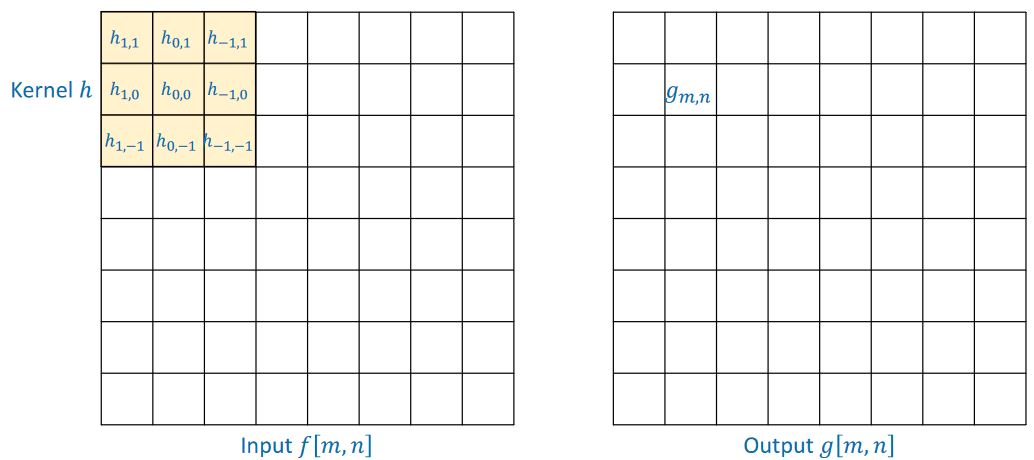
\includegraphics[width=8cm]{2D convolution.JPG}
\end{figure}

\subsection{Asspciativity and separable filters}

Note the associativity property of convolution:
$$
    f*(g*h) = (f*g)*h
$$
If a big filter can be separated as the convolution of two small filters, such
as $g*h$, then it is possible to first convolve $f$ with $g$ then with $h$.
$$
    f*filter_{big} = f*(g*h) = (f*g)*h
$$
\begin{figure}[h]
    \centering
    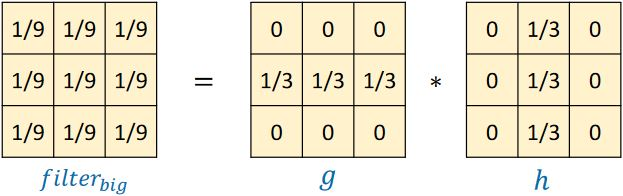
\includegraphics[width=8cm]{Associativity and separable.JPG}
\end{figure}

%%%%%%%%%%%%%%%%%%%%%%%%%%%%%%%%%%%%%%%%%%%%%%%%%%%%%%%%%%%%%%%%%%%%%%%%%%%%%%%%%%%%%%%%%%%%
\chapter{Edge Detection I}

In computer vision, an edge refers to lines where image brightness changes
sharply and has discontinuities. Edges capture important properties of the world
and are important low-level features for analysing and understanding images.

To detect edges, we note that an image can be regarded as a function of pixel
position. As known from mathematics, derivatives characterises the
discontinuities of a function which can be used to help detect edges. For
example, consider the definition of a continuous function:
$$
    f'(x) = \lim_{h \rightarrow 0} \frac{f(x+h) - f(x)}{h}
$$
\begin{figure}[h]
    \centering
    \subfloat[\centering Continuous function]{{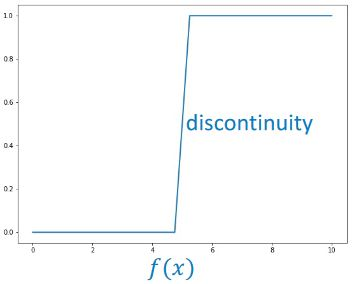
\includegraphics[width=5cm]{Edge derivative 1.JPG}}}%
    \qquad
    \subfloat[\centering Differentiated function showing detected discontinuity]{{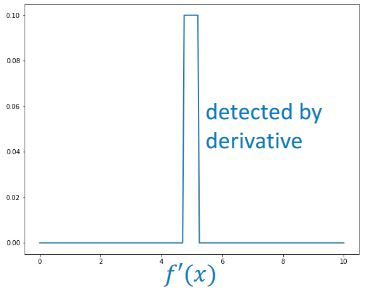
\includegraphics[width=5cm]{Edge derivative 2.JPG}}}%
\end{figure}
 
For a discrete function, the finite difference can be calculated using:
\begin{itemize}
    \item Forward difference: $f'[x] = f[x+1] - f[x]$
    \item Backward difference: $f'[x] = f[x] - f[x-1]$
    \item Central difference: $f'[x] = \frac{f[x+1] - f[x-1]}{2}$
\end{itemize}

This finite difference can be performed using convolution with kernals such as:
\begin{itemize}
    \item $h=[1,-1,0]$
    \item $h=[0,1,-1]$
    \item $h=[1,0,-1]$
\end{itemize}

\section{Convolution}

As mentioned earlier, convolution is often implemented:
$$
    g[n] = f[n] * h[n] = \sum_{m=-\infty}^\infty f[n-m]h[m] = \sum_{m=-\infty}^\infty f[n+m]h[-m]
$$

The \textit{central difference}, without accounting for $\frac{1}{2}$, can be
defined as:
\begin{align*}
    f'[x] &= f[x+1] - f[x-1] \\
    &= f[x+1] *1 + f[x] * 0 + f[x-1] * (-1) \\
    &= f[x+1] * h[-1] + f[x] * h[0] + f[x-1] * h[1] 
\end{align*}

The convolution kernal is this defined as: $h = [1,0,-1]$. The process of
convolution with central difference $f'[x] = f[x] * h[x]$ can be seen as shown below: 
\begin{figure}[h]
    \centering
    \subfloat{{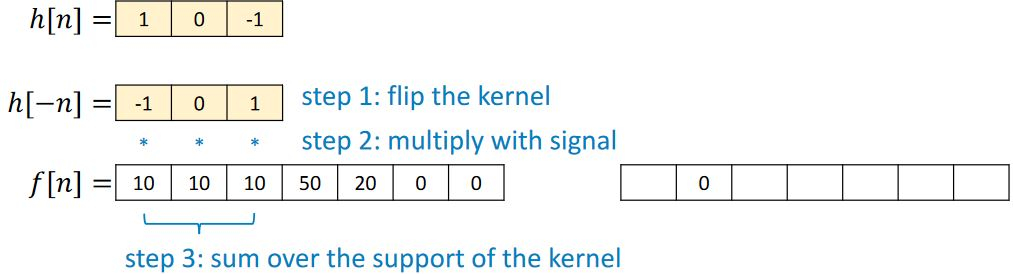
\includegraphics[width=8cm]{Edge convolution 1.JPG}}}%
    \qquad
    \subfloat{{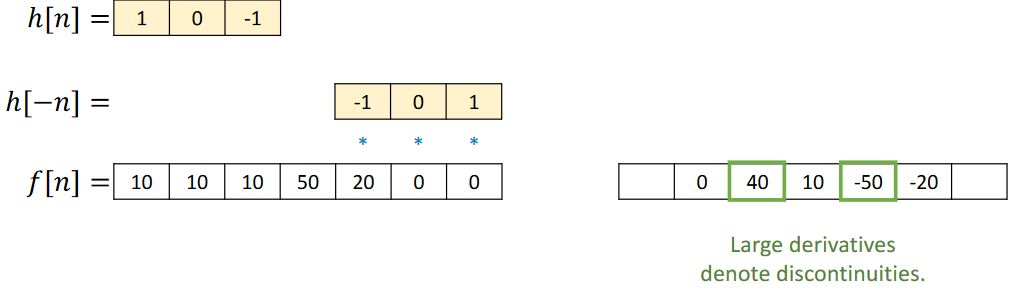
\includegraphics[width=8cm]{Edge convolution 2.JPG}}}%
\end{figure}

Note the following:
\begin{itemize}
    \item The kernal $h[n]$ is flipped $h[-n]$ as mentioned earlier on how
    convolution implemented
    \item Large derivatives denote discontinuities 
\end{itemize}

The following methods only enable discontinuities to be detected in 1D. Similar
filters have to be designed to extend edge detection to a 2D image.

\section{Edge detection filters}

\subsection{Prewitt filter}
\begin{figure}[h]
    \centering
    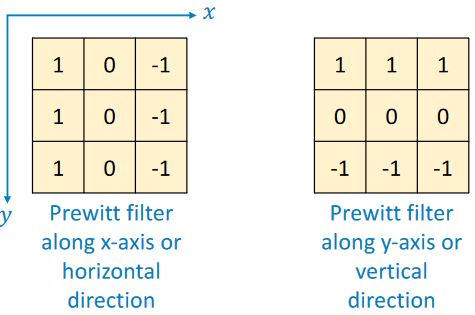
\includegraphics[width=5cm]{Prewitt.JPG}
    \hspace{2cm}
    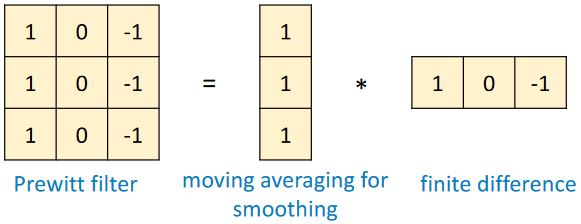
\includegraphics[width=6cm]{Prewitt separable.JPG}
\end{figure}

\subsection{Sobel filter}
\begin{figure}[h]
    \centering
    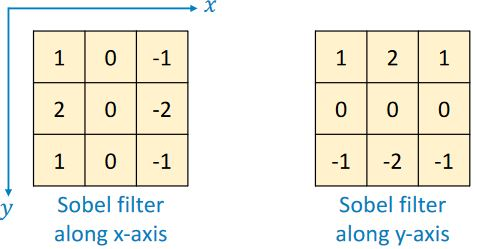
\includegraphics[width=5cm]{Sobel 1.JPG}
    \hspace{2cm}
    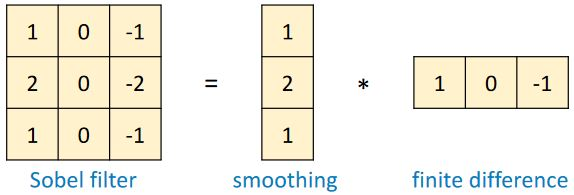
\includegraphics[width=6cm]{Sobel 2.JPG}
\end{figure}

\section{Image Gradient}

There are two outputs from Sobel filters that are combined to describe edges:
\begin{itemize}
    \item describing discontinuity along x-axis
    \item describing discontinuity along y-axis
\end{itemize}

The two outputs are combined to describe the two properties of edges: \textit{Magnitude} 
and \textit{Orientation} using the following process:
\begin{enumerate}
    \item Compute the derivatives along x-axis and y-axis:
    \begin{align*}
        g_x = f * h_x \\
        g_y = f * h_y
    \end{align*}
        
    \item Compute the magnitude of the gradient:
    $$
        g = \sqrt{g_x^2 + g_y^2}
    $$

    \item Compute the orientation or angle of the gradient:
    $$
        \theta = \arctan2(g_y, g_x)
    $$
\end{enumerate}

\section{Smoothing}

Derivatives are sensitive to noise thus using a smoothing kernel beforehand to
suppress the noise would result in a better result. This can be seen in the
Prewitt and Sobel filter which have a smoothing kernel built in. 

An alternative is to use the Gaussian kernel for smoothing before calculating
the derivatives. The following images show the ease of edge detection after
smoothing compared to no smoothing performed beforehand.
\begin{figure}[h]
    \centering
    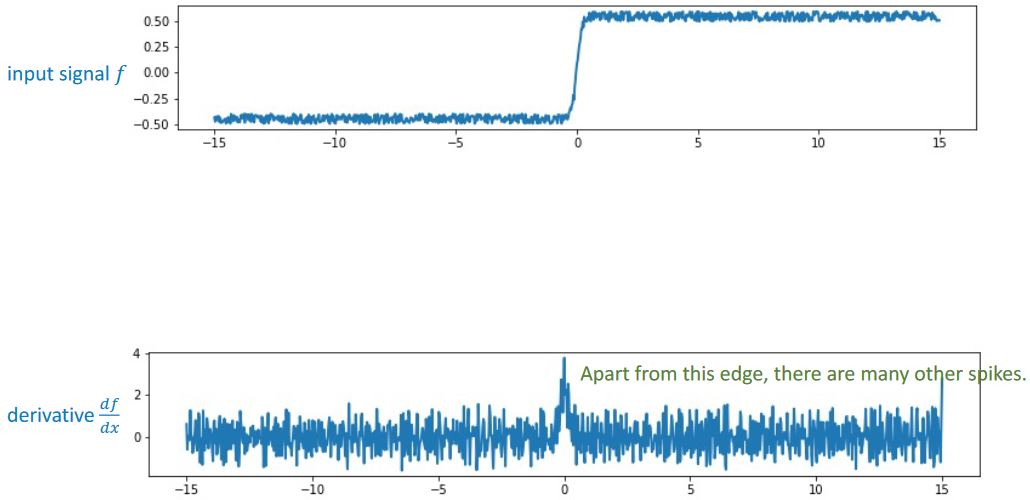
\includegraphics[width=8cm]{Smoothing 1.JPG}
    \hspace{1cm}
    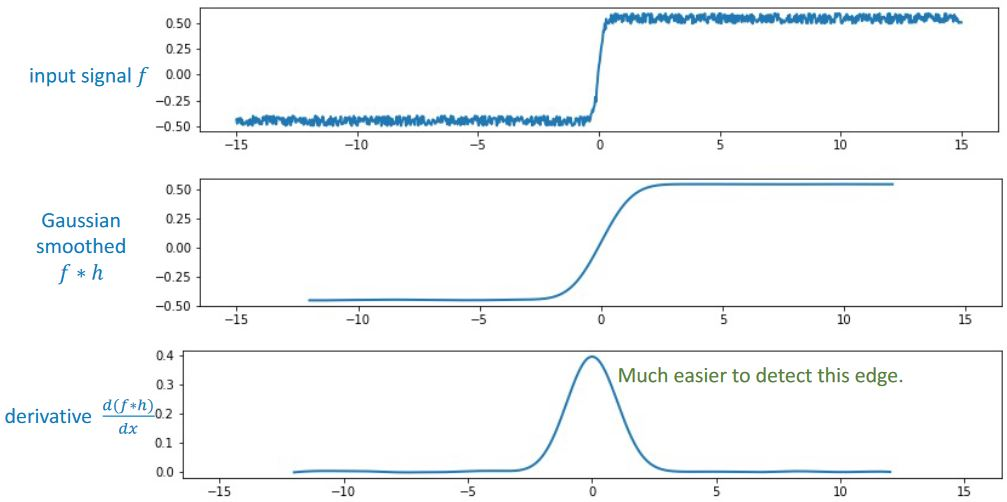
\includegraphics[width=8cm]{Smooth 2.JPG}
\end{figure}

\subsection{Derivative of Gaussian Filter}

\textit{Derivative of Gaussian filter} is an operator that performs Gaussian
smoothing before taking the derivative. 
\begin{gather*}
    g[x] = \frac{1}{\sqrt{2\pi} \sigma}e^{-\frac{x^2}{2\sigma^2}} \quad \text{Gaussian kernel} \\
    \frac{d}{dx}(f * h) \quad \text{Derivative of Gaussian filter}
\end{gather*}

Using the differentiation of convolution:
$$
    \frac{d}{dx}(f*h) = \frac{df}{dx} * h = f * \frac{dh}{dx} 
$$

The analytical form for the derivative of Gaussian kernel can be defined as:
\begin{figure}[h]
    \centering
    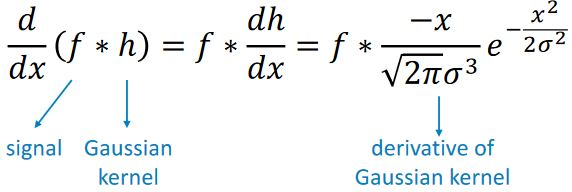
\includegraphics[width=5cm]{Gaussian derivative.JPG}
\end{figure}
\begin{figure}[h]
    \centering
    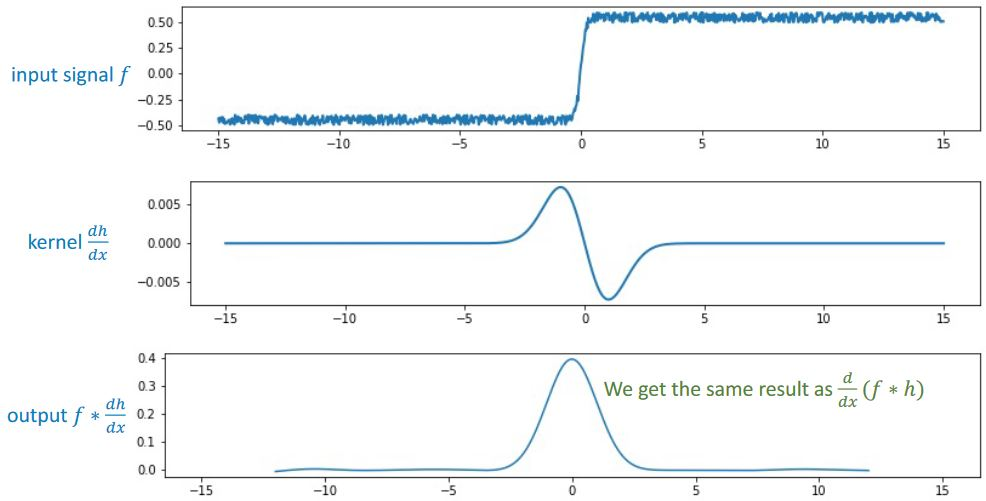
\includegraphics[width=9cm]{Derivative gaussian.JPG}
\end{figure}

\pagebreak

\begin{itemize}
    \item 1D Gaussian filter: $h[x] = \frac{1}{\sqrt{2\pi}\sigma} e^{-\frac{x^2}{2\sigma^2}}$ 
    \item 2D Gaussian filter: $h[x, y] = \frac{1}{2\pi\sigma^2} e^{-\frac{x^2 + y^2}{2\sigma^2}}$ 
\end{itemize}

It is a separable filter and equivalent to convolution of two 1D Gaussian
filters. This means that 2D Gaussian smoothing can be accelerated using
separable filtering. 

The process of a Gaussian Derivative Filter is defined as:
\begin{enumerate}
    \item Smooth the input image with a 2D Gaussian filter 
    \item Take the derivative along x-axis and y-axis 
    \item Calculate the magnitude and orientation 
\end{enumerate}

\subsubsection{Parameter $\sigma$ in derivative of Gaussian}
Large $\sigma$ value suppresses noise and results smoother derivative. Different
$\sigma$ values finds edges at different scales. 
\begin{figure}[h]
    \centering
    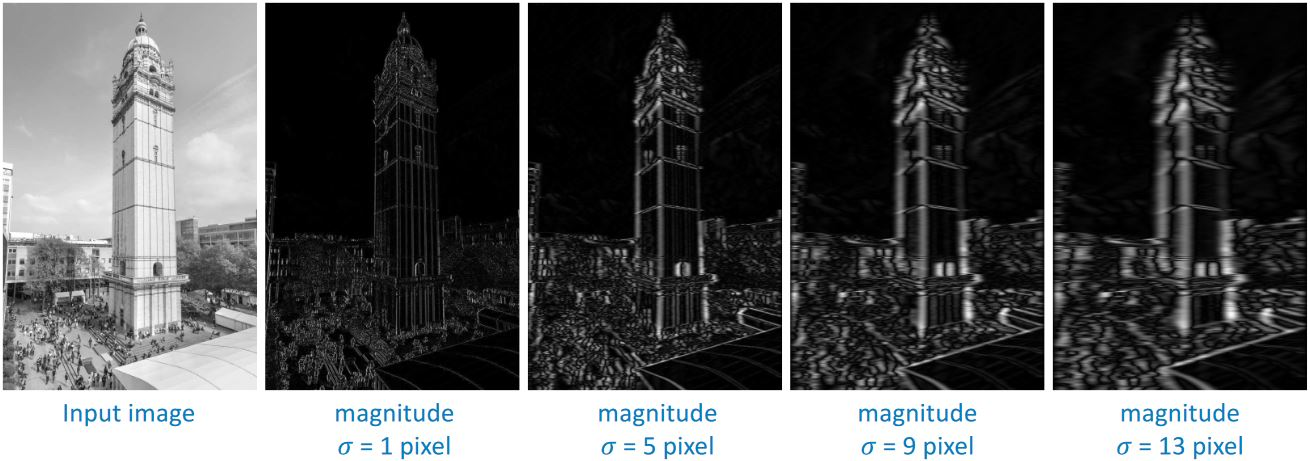
\includegraphics[width=12cm]{Gaussian derivative sigma.JPG}
\end{figure}
\chapter{Edge Detection II}

As mentioned earlier, edge detection is a fundamental problem in image
processing and computer vision that aims to identify points in an image that are
edges i.e. where discontinuities occur. 

There are two solutions to the problem:
\begin{itemize}
    \item \textbf{Canny approach}: Know explicitly the criteria of edge points,
    can design computational procedures to satisfy these 
    \item \textbf{Machine Learning}: Collect data which represent what to achieve e.g.
    manually drawn edge maps and train a machine learning model to map from images
    to final outputs.
\end{itemize}

\section{Canny Edge Detection}

John Canny defines a good edge detector:
\begin{itemize}
    \item \textbf{Good detection}: Low probability of failing to mark real edge
    points and falsely marking non-edge points 
    \item \textbf{Good localisation}: Points marked as edge points by operator
    should be as close as possible to the centre of the true edge 
    \item \textbf{Single response}: Only one response to a single edge 
\end{itemize}

Canny edge detection algorithm is summarised into the following:
\begin{enumerate}
    \item Perform Gaussian filtering to suppress noise
    \item Calculate the gradient magnitude and direction
    \item Apply \textit{non-maximum suppression} (NMS) to get a single response for each edge
    \item Perform \textit{hysteresis thresholding} to find potential edges
\end{enumerate}

\subsection{Gaussian filtering}

Gaussian filtering is performed to smooth image and suppress noise. The effect
of smoothing can be adjusted by the parameter $\sigma$ in the Gaussian kernel.
$$
    h(x,y) = \frac{1}{2\pi \sigma^2} e^{-\frac{x^2 + y^2}{2\sigma^2}}
$$

The effect of Gaussian smoothing parameter $\sigma$ on edge detection is:
\begin{figure}[h]
    \centering
    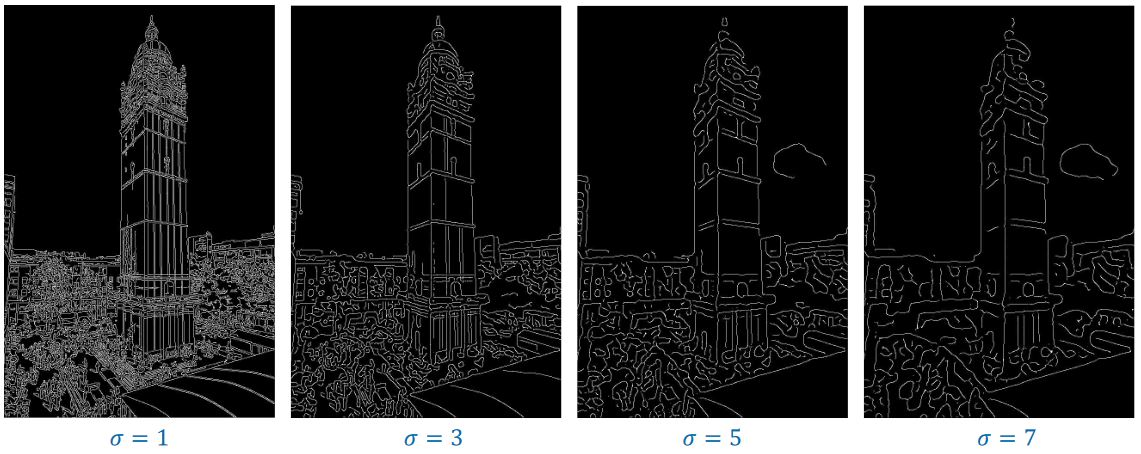
\includegraphics[width=8cm]{Gaussian smoothing.JPG}
\end{figure}

The choice of $\sigma$ depends on desired edge detection behavior:
\begin{itemize}
    \item Large $\sigma$: Detects large-scale edges and smooths out fine details.
    \item Small $\sigma$: Detects fine features.
\end{itemize}

\subsection{Image gradient}

The image gradient is calculated after Gaussian filtering. Common filters are
\textit{Prewitt} and \textit{Sobel}.

\subsection{Non-maximum suppression (NSM)}

The aim of NMS is to get a single response for an edge. The main concept of NMS:
Edge occurs where the gradient magnitude reaches the maximum. 

The NMS process is defined:
\begin{enumerate}
    \item Check whether a pixel $q$ is a local maximum along the gradient direction
    \item Move to pixel $r$ and compare the gradient magnitudes between $q$ and $r$
    \item Move to pixel $p$ and compare the gradient magnitudes between $q$ and $p$
    \item If pixel $q$ is the local maximum, it is an edge point and suppress
    the other pixels, i.e. non-maximum pixels
    $$
        M(x,y) = \begin{cases}
            M(x,y) & \text{if local maximum} \\
            0 & \text{otherwise}
        \end{cases}
    $$
\end{enumerate}

\begin{figure}[h]
    \centering
    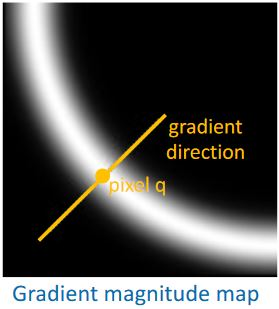
\includegraphics[width=3cm]{NMS_1.JPG}
    \hspace{1cm}
    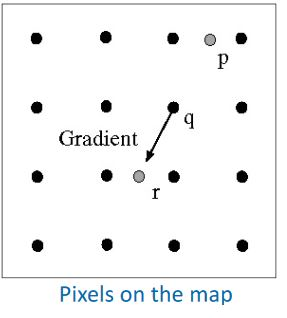
\includegraphics[width=3cm]{NMS_2.JPG}
\end{figure}

In implementation, we need to perform image interpolation for pixels $p$ and
$r$, if they are not located on the pixel lattice using nearest neighbour or
linear interpolation.

\subsection{Thresholding}

Thresholding is performed to ensure edges have high magnitudes. When performing
NMS for all pixels on the gradient magnitude map, many pixels may have low
magnitude even though it is a local maxima. 

The simplest thresholding methods replace each pixel in an image with a black
pixel if the image intensity $I_{i,j}$ is less than some fixed constant $T$
(that is $I_{i,j} < T$), or a white pixel if the image intensity is greater than that
constant. This is the method of segmenting images. 
$$
    \text{binary}(x,y) = \begin{cases}
        1 & \text{if} I(x,y) \leq t \\
        0 & \text{otherwise}
    \end{cases}
$$

From a grayscale image, thresholding can be used to create binary images. 
\begin{figure}[h]
    \centering
    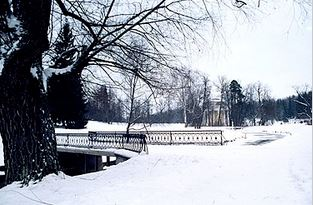
\includegraphics[width=5cm]{Thresholding_1.JPG}
    \hspace{1cm}
    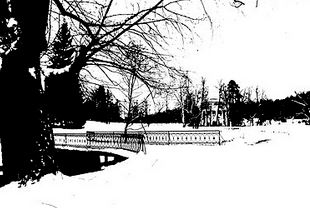
\includegraphics[width=5cm]{Thresholding_2.JPG}
\end{figure}

A common alternative is \textbf{Hysteresis thresholding} which is done by the
canny edge detector. 

\subsubsection{Hysteresis Thresholding}

Hysteresis thresholding defines two thresholds $t_{low}$ and $t_{high}$ for edge
detection:
\begin{itemize}
    \item If a pixel's gradient magnitude is $\leq t_{high}$, pixel is accepted as an edge pixel.
    \item If a pixel’s gradient magnitude is $< t_{low}$, pixel is rejected.
    \item If it is in between, it is a weak edge pixel i.e. may be an edge or may not be.
    \begin{itemize}
        \item Check neighbouring pixels, pixel is accepted if it is connected to an edge pixel
    \end{itemize}
\end{itemize}
\begin{figure}[h!]
    \centering
    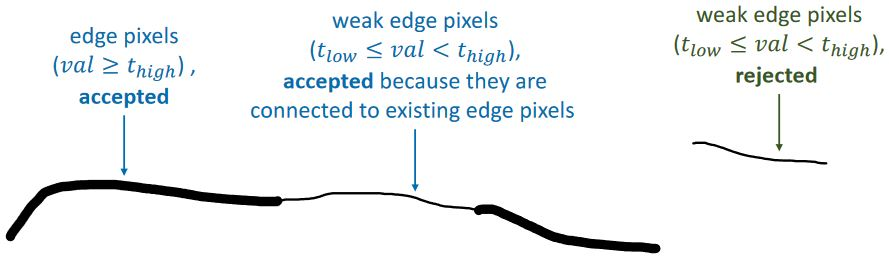
\includegraphics[width=7cm]{Hysteresis thresholding.JPG}
\end{figure}

The result can be seen in the image:
\begin{figure}[h]
    \centering
    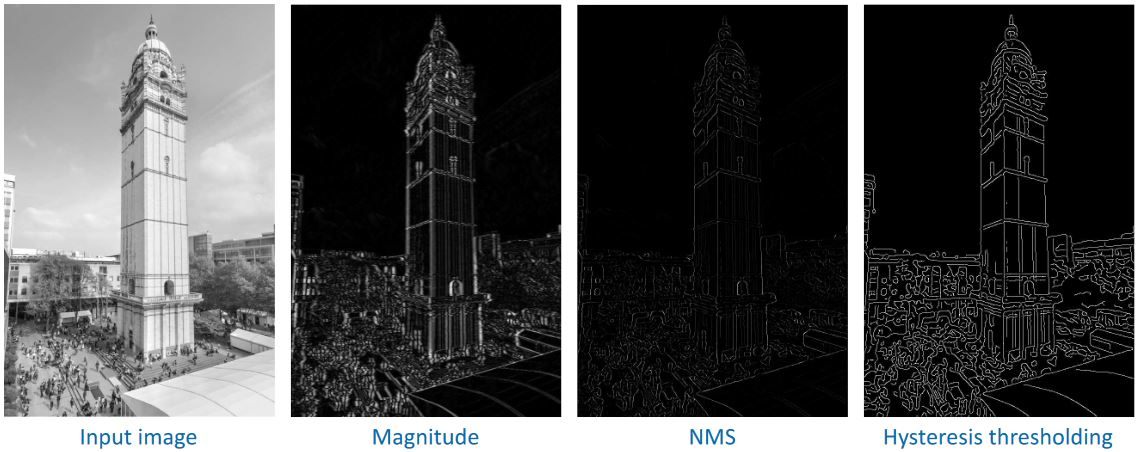
\includegraphics[width=9cm]{Process hysteresis.JPG}
\end{figure}

\subsection{Canny Edge Detection and its goals}

John Canny's initial goal is achieved by:
\begin{itemize}
    \item \textbf{Good detection}: 
    \begin{itemize}
        \item Gaussian smoothing to suppress noise (reducing false positives)
        \item Hysteresis thresholding to find weak edges (reducing false negatives)
    \end{itemize}
    \item \textbf{Good localisation}:
    \begin{itemize}
        \item Finding the location of edges using non-maximum suppression, which is based on gradient
        magnitude and direction
    \end{itemize}
    \item \textbf{Single response}:
    \begin{itemize}
        \item Non-maximum suppression (NMS)
    \end{itemize}
\end{itemize}

\section{Improving Edge Detection}

The Canny Edge Detection approach is designed by the following approach:
\begin{enumerate}
    \item Think of what criteria edges need to satisfy
    \item Carefully design the \textit{image features} (e.g. Gaussian filtering + image gradient)
    and \textit{procedures} (e.g. NMS, hysteresis thresholding) to achieve that criteria.
\end{enumerate}

There are many improvements that can be made in improving edge detection accuracy such as:
\begin{itemize}
    \item Utilising richer features, e.g. colour, texture
    \item Integrating multi-scale features
    \item Enforcing smoothness
    \item Machine learning, e.g. learning the mapping from image to edge directly from paired data
\end{itemize}

\subsection{Learning-based Edge detection}

Develop a machine learning model for edge detection based on:
\begin{itemize}
    \item Assuming that paired data (images $x$ + manually defined edge maps
    $y$) are available
    \item Common problem is how to find a model $f$ that maps $x$ to $y$, i.e. $y=f(x|\theta)$ , where
    $\theta$ denotes the model parameters
\end{itemize}

For example, consider this model:
\begin{figure}[h]
    \centering
    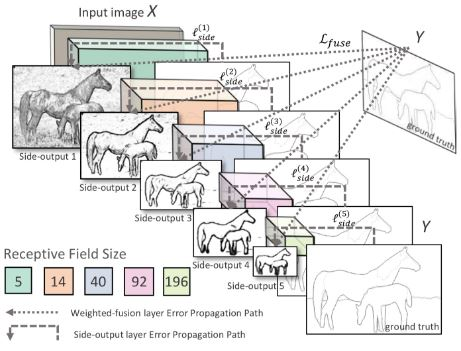
\includegraphics[width=8cm]{Learning-based approach.JPG}
    \caption{The colourful blocks are a machine learning model (e.g. neural
    network) that maps an input image into an edge map.}
\end{figure}

This machine learning model integrates features from multiple scales, fusing
fine-scale edges with coarse-scale edges to form the final output. This is
vastly different compared to the Canny edge detector which only uses a single
scale for edge detection, controlled by the Gaussian parameter $\sigma$.

%%%%%%%%%%%%%%%%%%%%%%%%%%%%%%%%%%%%%%%%%%%%%%%%%%%%%%%%%%%%%%%%%%%%%%%%%%%%%%%%%%%%%%%%%%%%
\chapter{Hough Transform}

With edge detection,a binary edge map which contains a lot of
edge points is obtained. If these edge points belong to a line, how is a parametric
representation of the line obtained? 

Hough transform is a transform from image space to parameter space e.g. from an
edge map to the two parameters of a line. The result is a parametric model,
given the input edge points. The aim of this transform is to detect shapes and
objects by a voting procedure.

Advantage:
\begin{itemize}
    \item It detects multiple instances.
    \item Robust to image noise.
    \item Robust to occlusion.
\end{itemize}

Limitations:
\begin{itemize}
    \item The computational complexity can be high. For each edge point, we need to vote to
    a 2D or even 3D parameter space.
    \item Need to carefully set some parameters, such as the parameters for the edge
    detector, the threshold for the accumulator or the range of circle radius
\end{itemize}

\section{Line parameterisation}

A line can be represented in several forms:
\begin{itemize}
    \item Slope intercept form: 
    $$
        y = mx + b
    $$
    where $m$ is the \textit{gradient} and $b$ is the \textit{y-axis intercept}

    \item Double intercept form: 
    $$
        \frac{x}{a} + \frac{y}{b} = 1
    $$
    where $a$ is the \textit{x-intercept} and $b$ is the \textit{y-intercept} 

    \item Normal form: 
    $$
        x\cos(\theta) + y\sin(\theta) = \rho
    $$
    where $\theta$ is the \textit{angle} and $\rho$ is the \textit{distance from origin}  
\end{itemize}

\section{Model fitting}

A common alternative to Hough transform is to fit a line model onto edge points:
\begin{itemize}
    \item Suppose there is set of points $(x_1, y_1), (x_2, y_2), \dots$ to fit
    a line model $y = mx + c$
    \item $m$ and $b$ can be estimated by minimising the fitting error: 
    $$
        \text{min}_{m,b} \sum_i [y_i - (mx_i + b)]^2
    $$
    where:
    \begin{itemize}
        \item $y_i$ - Real $y$ of a point 
        \item $mx_i + b$ - $\hat{y}$ estimated by our line model 
    \end{itemize}
\end{itemize}

\pagebreak

\section{Hough Transform}

Define the slope intercept form for a line model:
$$
    y = mx + b \rightarrow b = y - mx
$$

Each edge points in the image space $(x_1, y_1), (x_2, y_2), (x_3, y_3), ...$
votes for a line model in the parameter space e.g. the first point will vote
for $b = y_1 - mx_1$
\begin{figure}[h]
    \centering
    \includegraphics[width=10cm]{Hough transform.JPG}
\end{figure}

With this, the parameter space is divided into 2D bins where each point
increments the vote by 1 in one of the bins as seen below:
\begin{figure}[h]
    \centering
    \includegraphics[width=3cm]{Hough bins.JPG}
\end{figure}

The problem with the slope intercept form is that the parameter space is too
large where $m \in [-\infty, \infty]$ and $b \in [-\infty, \infty]$. Alot of
bins would be needed.

The solution is to use the \textit{normal form} $x\cos(\theta) + y\sin(\theta) =\
\rho$ where $\theta \in [0, \pi)$ and $\rho \in [-\infty, \infty]$. Note that
although $rho$ is infinite, it is technically limited by the image size.   
\begin{figure}[h]
    \centering
    \includegraphics[width=10cm]{Normal Hough.JPG}
    \caption{Conversion from \textit{slope intercept} to \textit{normal form}}
\end{figure}

\subsection{Line detection by Hough transform}

The algorithm is defined as:
\begin{enumerate}
    \item Initialise bins $H(\rho, \theta)$ to all zeros 
    \item For each edge point $(x,y)$:
    \begin{enumerate}
        \item For $\theta$ from $0$ to $\pi$: 
        \begin{itemize}
            \item Calculate $\rho = x\cos(\theta) + y\sin(\theta)$
            \item Accumulate $H(\rho, \theta) = H(\rho, \theta) + 1$
        \end{itemize}
    \end{enumerate}
    \item Find $(\rho, \theta)$ where $H(\rho, \theta)$ is a \textit{local maximum} and
    larger than a \textit{threshold} 
    \begin{itemize}
        \item Local maximum is chosen as it is similar to NMS in edge detection 
        \item Thresholding is required as a few random points would not lead to
        a line being detected 
    \end{itemize}
    \item Detected lines are defined by $\rho = x\cos(\theta) + y\sin(\theta)$
\end{enumerate}

This approach is different from model fitting where $(m,b)$ is defined by:
$$
    \text{min}_{m,b} \sum_i [y_i - (mx_i + b)]^2
$$
where only one line will be detected. 

\textbf{Shapes}: Unlike model fitting, Hough Transform can simultaneously detect multiple lines
as long as the lines are local maxima above a threshold. This allows Hough
transform to detect other shapes such as Ellipses, Planes in 3D space etc
\begin{figure}[h]
    \centering
    \includegraphics[width=10cm]{Hough ex1.JPG}
\end{figure}

\textbf{Noise}: Hough transform is robust to noise. An edge map is often generated after image
smoothing and broken edge points can still vote and contribute to line detection.
\begin{figure}[h]
    \centering
    \includegraphics[width=10cm]{Hough ex2.JPG}
\end{figure}

\textbf{Occlusion}: Hough transform is robust to object occlusion e.g. rectangle
covered by a bunny. The remaining edge points vote and contribute to line
detection. 
\begin{figure}[h]
    \centering
    \includegraphics[width=10cm]{Hough ex3.JPG}
\end{figure}

\section{Circle detection}

Hough Transform can be used to detect other shapes such as circles. The circle
canbe parameterised as:
$$
    (x-a)^2 + (y-b)^2 = r^2
$$
where the image space $(x,y)$ is transformed into the parameter space $(a,b,r)$. 

\pagebreak

\begin{figure}[h]
    \centering
    \includegraphics[width=10cm]{Circle.JPG}
\end{figure}

If the radius $r$ is known, then for each edge point $(x,y)$, there is only the
need to vote for possible values of $(a,b)$ i.e. still in parameter space $H(a,b)$. 

\section{Circle detection by Hough Transform}

The algorithm is defined as:
\begin{enumerate}
    \item Initialise the bins $H(a, b, r)$ to all zeros
    \item For each possible radius $r \in [r_{min}, r_{max}]$
    \begin{itemize}
        \item For each edge point $(x, y)$
        \begin{itemize}
            \item Let $\theta$ to be gradient direction, or opposite gradient direction
            \item Calculate $a = x - r\cos(\theta), b = y - r\sin(\theta)$
            \item Accumulate $H(a,b,r) = H(a,b,r) + 1$
        \end{itemize}
    \end{itemize}
    \item Find $(a,b,r)$ where $H(a,b,r)$ is a local maximum and larger than a threshold
    \item Detected circles are defined: $x = a + r\cos(\theta), y = b + r\sin(\theta)$
\end{enumerate}

\section{Generalised Hough Transform Idea}

\textbf{Weights}: When voting in the parameter space, it is possible to add
\textit{weights}. Instead of using equal vote for each edge point, the vote can be weighted
by the gradient magnitude so stronger edge points get higher weights.

\textbf{Spaces}:  There are two spaces, the image space and the parameter space
i.e. Hough space.
\begin{itemize}
    \item If the shape can be described by some parameters using an analytical equation, we
    use this equation to perform voting to the parameter space
    \item If it is not a simple shape without an analytical equation, as long as we have a model
    to describe it, we can still vote
\end{itemize}

%%%%%%%%%%%%%%%%%%%%%%%%%%%%%%%%%%%%%%%%%%%%%%%%%%%%%%%%%%%%%%%%%%%%%%%%%%%%%%%%%%%%%%%%%%%%
\chapter{Interest Point Detection I}

Interest points (keypoints, landmarks, low-level features) are image points
useful for subsequent image processing and analysis such as Image
classification, Image matching, Image retrieval etc. Interest points are mostly
corners or blobs, where local image structures are rich. 

\section{Facial Image Analysis}

A common use of interest points where interest points (landmarks) can be defined
to represent a face.
\begin{figure}[h]
    \centering
    \includegraphics[width=10cm]{Face interest points.JPG}
    \caption{Examples of landmarks representing a human face}
\end{figure}

These interest points are used to detect faces and the locations of interest
points can be used for mood analysis, augmented reality etc. 

\section{Image matching (Image alignment, Image registration)}

Image matching can be used to stitch images together by overlaying the matching
parts. The correspondance i.e. similarity between two images can be found using three methods:
\begin{itemize}
    \item Pixels: Using \textit{all} information 
    
    Optimising a similarity metric based on all image pixels:
    $$
        \text{max}_T Similarity(Image_A, Image_B(T))
    $$
    where $T$ denotes spatial transformation

    \begin{figure}[h!]
        \centering
        \includegraphics[width=8cm]{matching pixels.JPG}
    \end{figure}

    \pagebreak

    \item Edges: Using \textit{some} information 
    \begin{figure}[h!]
        \centering
        \includegraphics[width=8cm]{matching edges.JPG}
    \end{figure}

    \item Interest points: Using \textit{very little but important} information 
    \begin{figure}[h!]
        \centering
        \includegraphics[width=8cm]{matching interest point.JPG}
    \end{figure}
\end{itemize}

\section{Interest Point Detection}

Interest points are generally corners i.e. intersections of edges and the Harris Corner Detector is an
algorithm that could detect it.

\subsection{Harris Corner Detection}

Edge detection works by calculating the magnitude of image gradient at each
pixel. Edge pixels correspond to high magnitude of gradient.

The difference in corner detection is that edge detection methods could not
differentiation between edge and corner pixels. But, by using a small window,
the difference between edge pixels and corner pixels could be detected. 
\begin{figure}[h]
    \centering
    \includegraphics[width=10cm]{window dection.JPG}
\end{figure}

By shifting the window and calculating the change of intensities for the window:
\begin{itemize}
    \item \textbf{Edges}: Change of intensity along just one direction 
    \item \textbf{Corner}: Change of intensity along both direction
\end{itemize}

\pagebreak

Mathematics can be used to describe the change of pixel intensities in a given
window $W$. Given a window shifting by $[u, v]$, the change intensities is given by:
\begin{figure}[h]
    \centering
    \includegraphics[width=8cm]{Harris math.JPG}
\end{figure}
where the window function $w(x,y)$ can be a Step or Gaussian function  

\subsection{Change of Intensities}

A small shift $[u,v]$ is defined with the following bilinear approximation 
$$
    E(u,v) \approx [u,v] . M . \begin{bmatrix}
        u \\
        v
    \end{bmatrix}
$$
where $M$ is a $2 \times 2$ matrix derived from the window function and product
of image derivatives 
$$
    M = \sum_{x,y} w(x,y) \begin{bmatrix}
        I_x^2 & I_x I_y \\ 
        I_x I_y & I_y^2
    \end{bmatrix}
$$

Based on $
E(u,v) \approx [u,v] . M . \begin{bmatrix}
    u \\
    v
\end{bmatrix}
$: 
\begin{figure}[h]
    \centering
    \includegraphics[width=4cm]{Flat.JPG}
    \hspace{1cm}
    \includegraphics[width=4cm]{Edge.JPG}
    \hspace{1cm}
    \includegraphics[width=4cm]{Corner.JPG}
\end{figure}
\begin{itemize}
    \item $M = \begin{bmatrix}
        0 & 0 \\ 
        0 & 0
    \end{bmatrix}$: Flat region 

    \item $M = \begin{bmatrix}
        10 & 0 \\ 
        0 & 0.1
    \end{bmatrix}$: Edge - A large change if shifting window along $u$ but little
    change along $v$ 

    \item $M = \begin{bmatrix}
        10 & 0 \\ 
        0 & 10
    \end{bmatrix}$: Corner - A large change whichever way window shift occurs 
\end{itemize}

If $M$ is more complicated, the matrix $M$ can be made simpler by performing
eigen decomposition by using the face that eigenvectors are orthogonal to each
other. Since $M$ is a real symmetrical matrix, $M$ can be
decomposed by 
\begin{figure}[h]
    \centering
    \includegraphics[width=6cm]{decomposition.JPG}
\end{figure}

\pagebreak
\subsection{Intepreting Eigenvalues}

Getting the two eigen values of hessian matrix for all points will show the
category of that point.  
\begin{figure}[h]
    \centering
    \includegraphics[width=7cm]{Corner eigen.JPG}
\end{figure}

Corners are defined by eigenvalues are defined variously such as $R = \lambda_1
\lambda_2 - k(\lambda_1 + \lambda_2)^2$, $R = \text{min}(\lambda_1, \lambda_2)$,
$R= \frac{\lambda_1 \lambda_2}{\lambda_1 + \lambda_2 + \in}$, etc

\subsection{Cornerness}

Since only the values $\lambda_1 \lambda_2$ and $\lambda_1 + \lambda_2$, there
is no need to perform eigen-decomposition. Instead the properties of matrix
determinant and trace of $M = P \Lambda P^T$ defined as:
$$
    R = \text{det}(M) - k(\text{trace}(M))^2
$$
can be used:
\begin{gather*}
    \text{det}(M) = \text{det}(P \Lambda P^T) = \text{det}(\Lambda) = \lambda_1 \lambda_2 \\ 
    \text{trace}(M) = \text{trace}(P \Lambda P^T) = \text{trace}(\Lambda) = \lambda_1 + \lambda_2
\end{gather*} 

\section{Harris Detector}

This detector finds strong responses at corners, blobs and textures.
\begin{figure}[h]
    \centering
    \includegraphics[width=8cm]{Harris detector.JPG}
\end{figure}

Algorithm:
\begin{enumerate}
    \item Compute $x$ and $y$ derivatives of an image 
    \begin{gather*}
        I_x = G_x * I \\ 
        I_y = G_y * I
    \end{gather*}
    
    \item At each pixel, compute the matrix $M$
    \begin{gather*}
        M = \sum_{x,y} w(x,y) \begin{bmatrix}
            I_x^2 & I_x I_y \\ 
            I_x I_y & I_y^2
        \end{bmatrix}
    \end{gather*}

    \item Calculate the detector response 
    $$
        R = \lambda_1 \lambda_2 - k(\lambda_1 + \lambda_2)^2
    $$

    \item Detect interest points which are local maxima and whose response $R$
    are above a threshold.
\end{enumerate}

\subsection{Properties}

\textbf{Invariant to rotation}: Harris detector is rotation-invariant i.e. if a
corner is rotated, you can still get the same change of intensities when you
shift the window along a rotated direction. 

\textbf{Not invariant to scale}: Harris corner detector is not invariant to
scale. However, we can apply Harris detector at multiple scales and find the
response at the most suitable scale.

Multi-scale images are obtained through:
\begin{itemize}
    \item Gaussian smoothing with different $\sigma$
    \item Sampling with different spatial resolutions
\end{itemize}

%%%%%%%%%%%%%%%%%%%%%%%%%%%%%%%%%%%%%%%%%%%%%%%%%%%%%%%%%%%%%%%%%%%%%%%%%%%%%%%%%%%%%%%%%%%%
\chapter{Interest Point Detection II}

\section{Scale}

The Harris detector is not invariant to scale as seen in this following example:
\begin{figure}[h]
    \centering
    \includegraphics[width=4cm]{Harris scale.JPG}
\end{figure}

Different scales are required as images convolved with Gaussian kernels of
different $\sigma$ provide information at different scale as seen below:
\begin{figure}[h]
    \centering
    \includegraphics[width=14cm]{Harris different scale.JPG}
    \caption{Harris detector response when different Gaussian kernels are used for calculating image derivatives}
\end{figure}

How the scale is determined at each pixel is the problem. The goal is to be able
to choose a scale such that the region that looks most like a corner
\textbf{results in a high Harris detector response}.

\subsection{Response at different scales}

The Harris detector response is calculated using the eigenvalues of $M$
$$
    M = \sum_{x,y} w(x,y) = \begin{bmatrix}
        I_x^2(\sigma) & I_x(\sigma) I_y(\sigma) \\ 
        I_x(\sigma) I_y(\sigma) & I_y^2(\sigma)
    \end{bmatrix}
$$
which are in turn determined by the derivatives $I_x(\sigma)$ and $I_y(\sigma)$.
The derivatives are inversely proportional to scale $\sigma$  i.e. the larger
the scale $\sigma$, the smaller the derivatives magnitude.

\pagebreak

\subsection{Derivatives at different scales}

Consider two signals $f(x)$ and $g(x)$ which are related by $f(x) = g(sx)$ i.e.
only differing by scale $s$ and have the same peak magnitude.  This can happen,
for example, when a picture of the same object is taken with different zoom
factors.  
\begin{figure}[h]
    \centering
    \includegraphics[width=12cm]{Different zoom.JPG}
\end{figure}

The peak magnitudes of the calculated derivatives differ as well
\begin{figure}[h]
    \centering
    \includegraphics[width=12cm]{Derivative peak.JPG}
\end{figure}

The relationship between the two derivatives are defined as:
$$
    \frac{df}{dx} = s . \frac{dg}{dx} |_{sx}
$$
This equation shows that to make the derivative magnitude comparable across
scales, multiply the derivative by its scale $s$. The same object will give same
magnitude of response, regardless of the zoom factor.

\subsection{Scale adapted Harris detector}

The scale adapted Harris detector is defined as 
$$
    M = \sum_{x,y} w(x,y) \begin{bmatrix}
        \sigma^2 I_x^2(\sigma) & \sigma^2 I_x(\sigma) I_y(\sigma) \\
        \sigma^2 I_x(\sigma)I_y(\sigma) & \sigma^2 I_y^2(\sigma)
    \end{bmatrix} = \sum_{x,y}w(x,y) \sigma^2 \begin{bmatrix}
        I_x^2(\sigma) & I_x(\sigma) I_y(\sigma) \\
        I_x(\sigma)I_y(\sigma) &  I_y^2(\sigma)
    \end{bmatrix}
$$

At each pixel, determine the scale which gives the largest detector response (e.g. at this scale, it looks most like a corner)

The \textit{scale adapted Harris detector} composes of two steps:
\begin{itemize}
    \item Calculates the scale adapted detector response for a series of
    $\sigma$, from small-scale to large-scale
    
    \item Perform interest point detection and look for local maxima both
    across space and across scale
\end{itemize}

The algorithm, \textbf{for each $\sigma$}, is defined as:
\begin{enumerate}
    \item Perform Gaussian smoothing with $\sigma$
    \item Calculate the $x$ and $y$ derivatives of the smoothed image
    $I_x(\sigma)$ and $I_y(\sigma)$
    \item At each pixel, compute the matrix $M$
    $$
        M = \sum_{x,y}w(x,y) \sigma^2 \begin{bmatrix}
            I_x^2(\sigma) & I_x(\sigma) I_y(\sigma) \\
            I_x(\sigma)I_y(\sigma) &  I_y^2(\sigma)
        \end{bmatrix}
    $$
    \item Calculate the detector response
    $$
        R = \lambda_1 \lambda_2 - k(\lambda_1 + \lambda_2)^2
    $$
    \item Detect interest points which are local maxima across both scale and space
    and whose response $R$ are \textbf{above a threshold}.
\end{enumerate}

\section{Other interest point detectors}

\subsection{Laplacian of Gaussian (LoG)}

The Laplacian is the sum of second derivatives. For 2D image, it is
$$
    \Delta f = \bigtriangledown^2 f = \frac{\sigma^2 f}{\sigma x^2} + \frac{\sigma^2 f}{\sigma y^2}
$$
\begin{figure}[h]
    \centering
    \includegraphics[width=8cm]{Laplacian.JPG}
\end{figure}

Note that the second derivative is more sensitive to noise. For this reason, the
image is smoothed using a Gaussian kernel before calculating the Laplacian. 
\begin{gather*}
    \text{Laplacian: } \Delta f = \frac{\sigma^2 f}{\sigma x^2} + \frac{\sigma^2 f}{\sigma ^2y} \\
    \text{LOG: } \Delta(f*h) = \frac{\sigma^2(f*h)}{\sigma x^2} + \frac{\sigma^2 (f*h)}{\sigma y^2}
\end{gather*}

The analytical form for the LoG kernel is defined as:
\begin{gather*}
    \text{LoG: } \Delta(f*h) = \frac{\sigma^2(f*h)}{\sigma x^2} + \frac{\sigma^2(f*h)}{\sigma y^2} = f*\left(\frac{\sigma^2 h}{\sigma x^2} + \frac{\sigma^2 h}{\sigma y^2}\right)
\end{gather*}

Noting that 2D Gaussian is defined as $h(x,y) = \frac{1}{2\pi \sigma^2}
e^{-\frac{x^2 + y^2}{2\sigma^2}}$, the LoG can be derived 
\begin{gather*}
    \frac{\sigma^2 h}{\sigma x^2} + \frac{\sigma^2 h}{\sigma y^2} = -
    \frac{1}{\pi \sigma^4} \left(1 - \frac{x^2 + y^2}{2\sigma^2}\right) e^{-\frac{x^2 + y^2}{2\sigma^2}}
\end{gather*}

Similarly to Harris detector, if we want to determine the optimal scale at
each pixel, we need to make sure the LoG response is comparable between
scales. 

The LoG response at scale $\sigma$ is defined as:
$$
    LoG(x,y,\sigma) = I_{xx}(x,y,\sigma) + I_{yy}(x,y,\sigma)
$$

The normalised LoG response at scale $\sigma$ is defined as:
$$
    LoG_{norm}(x,y,\sigma) = \sigma^2(I_{xx}(x,y,\sigma) + I_{yy}(x,y,\sigma))
$$

\subsection{Difference of Gaussian (DoG)}

Difference of Gaussians (DoG) filter is defined as
$$
    DoG(x,y,\sigma) = I * G(k \times \sigma) - I * G(\sigma)
$$
where $k$ is a arbitary constant e.g. $k=\sqrt{2}$

DoG approximates the normalised Laplacian of Gaussian (LoG)
$$
    LoG_{norm}(x,y,\sigma) = \sigma^2(I_{xx}(x,y,\sigma) + I_{yy}(x,y,\sigma))
$$

DoG is a good approximation to the normalised Laplacian of Gaussian (LoG). It
provides some convenience in calculating the response across different
scales. 

\subsection{Summary of interest point detectors}
\begin{itemize}
    \item Scale-variant
    \begin{itemize}
        \item Harris detector
    \end{itemize}

    \item Scale-invariant
    \begin{itemize}
        \item Scale adapted Harris detector
        \item Normalised Laplacian of Gaussian
        \item Difference of Gaussian
    \end{itemize}

    The scale-invariant detectors follow similar procedures:
    \begin{itemize}
        \item Calculate the detector response across scales
        \item Find local extrema both across scale and across space
    \end{itemize}
\end{itemize}

\begin{figure}[h]
    \centering
    \includegraphics[width=11cm]{Interest point summary.JPG}
\end{figure}

%%%%%%%%%%%%%%%%%%%%%%%%%%%%%%%%%%%%%%%%%%%%%%%%%%%%%%%%%%%%%%%%%%%%%%%%%%%%%%%%%%%%%%%%%%%%
\chapter{Feature Description I}

Feature description describes the feature for each point so that the points can
be compared and matched. 

\section{Descriptors}

There are several types of descriptors:
\begin{itemize}
    \item Pixel intensity
    \item Patch intensities 
    \item Gradient orientation 
    \item Histogram 
    \item SIFT descriptor
\end{itemize}

\subsection{Pixel intensity}

Describes features using intensity of a single pixel. 

Problems:
\begin{itemize}
    \item Sensitive to absolute intensity value. Intensity of the same point
    will change under different illumination.  
    \item Not discriminative. The grayscale intensity ranges from 0 to 255. There are
    thousands of pixels with exactly the same intensity.
\end{itemize}

\subsection{Patch intensities}

Better than single pixel intensity and represents the local pattern. This
performs well if the images are of similar intensities and roughly aligned. 

\textbf{Problems}:
\begin{itemize}
    \item Sensitive to absolute intensity value 
    \item Not rotation-invariant 
\end{itemize}

\subsection{Gradient orientation}

This type is robust to changes in intensity. 

\textbf{Problem}:
\begin{itemize}
    \item Not rotation invariant 
\end{itemize}

\subsection{Histogram}

The intensity histogram of a patch. This is robust ot rotation and scaling. 

\textbf{Problem}:
\begin{itemize}
    \item Sensitive to intensity changes 
\end{itemize}

\section{SIFT algorithm}

Combination of the gradient orientation (robust to intensity changes) and
histogram (robust to rotation and scaling). The algorithm is used for detecting
and describing local features in images. 

This algorithm transforms an image into a large set of interest points, each of which is
described by a feature vector that is invariant to translation, scaling and
rotation.

The SIFT algorithm is defined into the following steps:
\begin{enumerate}
    \item Detection of scale-space extrema [Detection]
    \item Keypoint localisation 
    \item Orientation assignment [Description] 
    \item Keypoint descriptor 
\end{enumerate}

\subsection{Detection of scale-space extrema}

Search across scales and pixel locations, looking for interest points.
Difference of Gaussian (DoG) filter is used to identity potential interest
points.
$$
    DoG(x,y,\sigma) = I * G(k \sigma) - I * G(\sigma)
$$

The difference of Gaussian for different scales $\sigma$ is calculated from fine
to coarse e.g. $\sigma, \sqrt{2}\sigma, 2\sigma, ...$. This is implemented as
first calculating a stack of Gaussian smoothed images then calculating their
differences.
\begin{figure}[h]
    \centering
    \includegraphics[width=10cm]{G to DoG.JPG}
\end{figure}

\subsection{Keypoint localisation}

SIFT can be improved to refine the localisation and scale by fitting a model
onto nearby data which can improve the accuracy for image matching:
\begin{itemize}
    \item A quadratic function is fitted to the DoG response of neighbouring pixels  
    \item Location and scale of extremum for this quadratic function can be
    estimated 
\end{itemize}

Denote the DoG response by $D(x,y,\sigma)$ or $D(x)$ where $x = (x,y,\sigma)^T$
is a 3D vector containing both location and scale. The refined estimate is
defined as: 
$$
    \Delta x = - \frac{\partial^2 D}{\partial x^2}^{-1} \frac{\partial D}{\partial x} 
$$
\begin{figure}[h]
    \centering
    \includegraphics[width=8cm]{Keypoint.JPG}
\end{figure}

\subsection{Orientation assignment}

Assigns a consistent orientation to each keypoint, based on local image
properties. As a result, the feature descriptor can be represented relative to
this orientation and achieve invariance to image rotation.

The key idea being that if the orientation of the image, it is possible to
sample in a rotated coordinate system before calculating features. The dominant
orientation $\theta$ for a neighbourhood of a keypoint found by:
\begin{itemize}
    \item Calculate the gradient orientation for pixels in this
    neighbourhood 
    \item An orientation histogram with 36 bins covering 360 degrees is
    created 
    \item Each pixel votes for an orientation bin, weighted by the gradient
    magnitude 
    \item Keypoint will be assigned an orientation that is the peak of the
    histogram 
\end{itemize}

\subsection*{Local image descriptor}

With sample points, it is possible to describe the local image content through:
\begin{itemize}
    \item Pixel intensities 
    \item Gradient orientations 
    \item Histograms 
\end{itemize}

SIFT uses the histogram of gradient orientations:
\begin{itemize}
    \item Calculate the gradient magnitudes and orientations for these sampling
    points. Orientations are calculated relative to the dominant orientation $\theta$
    \item Create a histogram of gradient orientations
\end{itemize}

In practice, \textit{subregions} are used and each subregion has $4 \times 4$ samples:
\begin{itemize}
    \item Each subregion will have one orientation histogram
    \item Obtain a number of histograms, which together describe what it looks
    like around the keypoint
\end{itemize}

\begin{figure}[h]
    \centering
    \includegraphics[width=8cm]{local image 1.JPG}
    \hspace{1cm}
    \includegraphics[width=8cm]{local image 2.JPG}
\end{figure}

This descriptor is robust to rotation, scaling and change of illuminations:
\begin{itemize}
    \item Consideration of dominant orientation
    \item A sampling window proportional to scale
    \item Use of gradient orientations for feature description
    \item Use of histograms
\end{itemize}

\subsection{Keypoint matching}

Keypoints between two images are matched by identifying the nearest neighbours:
\begin{itemize}
    \item For each keypoint in image A, identify its nearest neighbours in the database of
    keypoints for image B
    \item The distance is defined by the Euclidean distance of SIFT descriptors
\end{itemize}

The exact neighbours do not need to be found. There are faster algorithms for
finding approximate nearest neighbours.

\pagebreak

After nearest neighbour search, a keypoint is found $(x,y)$ in image A
corresponds to another keypoint $(u,v)$ in image B, the images are related by an
affine transformation:
\begin{figure}[h!]
    \centering
    \includegraphics[width=5cm]{affine.JPG}
\end{figure}

For many pairs of corresponding keypoints, the equation can be written as a
linear system
$$
    Am = b
$$
where $m$ - unknown affine parameters 

The least-square solution to the linear system is defined by the Moore-Penrose inverse:
$$
    m = (A^T A)^{-1} A^T b
$$
which minimises the squared difference $||Am - b||^2$

Once the affine parameters are solved, we know the spatial transformation between the two images.

\section{RANSAC}

The squared difference $||Am - b||^2$ is sensitive to outliers. To improve the robustness of matching, we can
employ methods which consider outliers in model fitting, such as Random Sample
Consensus (RANSAC).

For each iteration:
\begin{enumerate}
    \item Select random sample points 
    \item Fit a model 
    \item Based on the model, check how many points are inliers 
    \item Terminate after a certain number of iterations or enough inliners have been
    found 
\end{enumerate}

%%%%%%%%%%%%%%%%%%%%%%%%%%%%%%%%%%%%%%%%%%%%%%%%%%%%%%%%%%%%%%%%%%%%%%%%%%%%%%%%%%%%%%%%%%%%
\chapter{Feature Description II}

\end{document}   